\documentclass[11pt,a5paper,twoside]{book}
%format A5
%\usepackage[top=25mm, bottom=20mm, outer=20mm, inner=25mm]{geometry}
%Format Royal
\usepackage[paperwidth=156mm, paperheight=234mm,top=25mm, bottom=20mm, outer=20mm, inner=25mm]{geometry}
\usepackage[utf8]{inputenc}
\usepackage{graphicx}
\usepackage[english]{babel}
%Include des macros Pinyin pour traitement de-macro avant pandoc ou tex4ebook
\usepackage{Pinyin-private}
\usepackage[abs]{overpic}
\usepackage{color}
\usepackage{anyfontsize}
%=============================================================
\title{\TAIJIJIAN{}\\\Taiji{} sword fencing}
\author{Frédéric Plewniak}
\setlength\unitlength{1mm}
\begin{document}
%\newgeometry{top=0mm, bottom=0mm, outer=0mm, inner=0mm, hoffset=-6mm,voffset=0mm}
%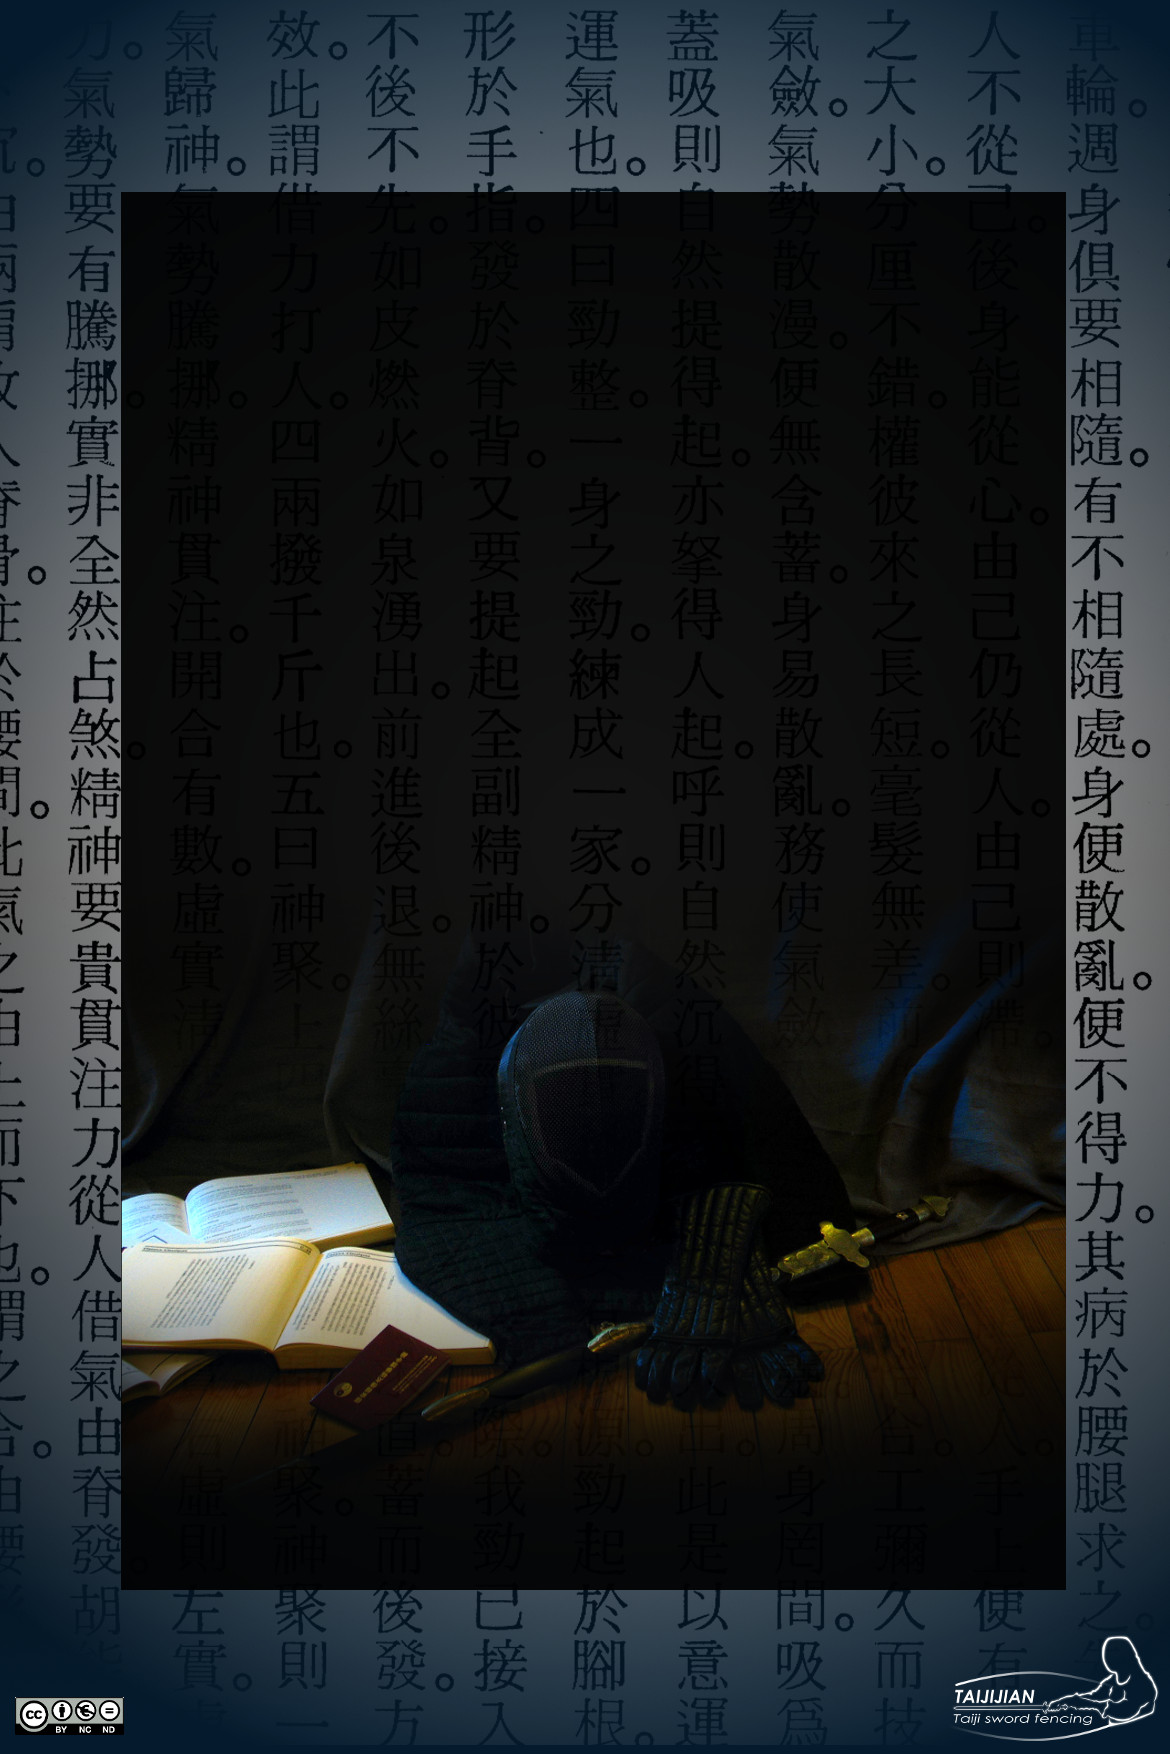
\includegraphics[width=\paperwidth]{../../Images/CouverturePDF_Royal}
\newgeometry{top=0mm, bottom=0mm, outer=0mm, inner=0mm, hoffset=-6mm,voffset=1mm}
\begin{overpic}[width=\paperwidth]%
{../../Images/CouverturePDF_Royal}
\put(28,180){\color{white}{{\upshape\fontfamily{ppl}\fontseries{b}\fontsize{50}{60}\selectfont \TAIJIJIAN{}}}}
\put(30,165){\color{white}{{\upshape\fontfamily{ppl}\fontseries{l}\fontsize{32}{30}\selectfont \Taiji{} sword fencing}}}

\put(70,25){\color{white}{{\scshape\fontfamily{pbk}\fontseries{l}\fontsize{20}{20}\selectfont Frédéric Plewniak}}}
\end{overpic}
\newpage
\mbox{ }
\end{document}